\documentclass[12pt]{article}
\usepackage[margin=1in]{geometry}
\usepackage[all]{xy}


\usepackage{amsmath,amsthm,amssymb,color,latexsym}
\usepackage{geometry}        
\geometry{letterpaper}    
\usepackage{graphicx}
\usepackage[russian]{babel}
\newtheorem{problem}{Задача}

\newenvironment{solution}[1][\it{Решение}]{\textbf{#1. } }{$\square$}
\newtheorem{theorem}{Теорема}[section]
\newtheorem{corollary}{Corollary}[theorem]
\newtheorem{lemma}[theorem]{Lemma}
\DeclareMathOperator{\Ima}{Im}
\DeclareMathOperator{\Kera}{Ker}

\begin{document}
\noindent ОВАиТК 2024\hfill Домашнее задание 6 \\
Гаттаров Тимур Б05-304 (13/03/2024)

\hrulefill

\begin{problem}
    $AB$
\end{problem}
\begin{problem}
    Построить гомоморфизм $\varphi$ аддитивной группы рациональных чисел $(\mathbb{Q},+)$, ядром которого является подгруппа целых чисел $(\mathbb{Z},+)$.
\end{problem}

\begin{solution}
    Построим гомоморфизм $\varphi$ из $(\mathbb{Q}, +)$ в группу корней из единицы $(A, \cdot)$ по следующему правилу:

    $$
    \forall q \in \mathbb{Q} \text{ } \exists \text{ } m \in \mathbb{Z}, n \in \mathbb{N} : q = \frac{m}{n} \hookrightarrow \varphi(q) = \varphi (m/n) = \cos{(2\pi m / n)} + i\sin{(2 \pi m / n)}
    $$

    Тогда имеем: 

    $$
    \forall z \in \mathbb{Z} \hookrightarrow \varphi(z) = \cos{(2\pi z)} + i\sin{(2 \pi z)} = 1 = e,
    $$

    где $e = 1$ - нейтральный элемент в $(A, \cdot)$. Таким образом, получаем $\Ker \varphi = (\mathbb{Q}, +).$
\end{solution}


\begin{problem}
    В предыдущей задаче покажите, что факторгруппа по ядру гомоморфизма имеет бесконечный порядок, но порядок каждого элемента конечен.
\end{problem}

\begin{solution}
    По основной теореме о гомоморфизмах: 
    $$
    G / Ker \varphi \cong \Ima \varphi
    $$

    В нашем случае имеем:
     $$
     (\mathbb{Q}, +) / \Kera \varphi \cong (A, \cdot),
     $$

    но группа $(A, \cdot)$ является бесконечной.
 Оценим порядок элемента, откуда сделаем вывод о его конечности:
    $$
    |\cos{(2\pi m / n)} + i\sin{(2 \pi m / n)}| \leq n \in \mathbb{Z}.
    $$
\end{solution}


\begin{problem}
     Покажите, что факторгруппа невырожденных матриц по умножению по подгруппе матриц с детерминантом 1 изоморфна мультипликативной группе действительных чисел $(\mathbb{R} \backslash\{0\}, \times)$.
\end{problem}

\begin{solution}
    Рассмотрим отображение $\varphi (A) = \det (A)$. Покажем,
    что $\varphi$ действительно является гомоморфизмом:
    По опрдеделению гомоморфизма: 
    $$ 
    \varphi - \text{гомоморфизм} \Leftrightarrow \displaystyle \varphi(x\cdot y)=\varphi(x) \cdot \varphi(y)
    $$
    По свойству детерминанта, доказанного в курсе Линейной алгебры:
    $$
    \det(A \cdot B) = \det (A) \cdot \det(B)
    $$

    Далее применим следующую теорему:
    
    \textit{(Основная теорема о гомоморфизмах) Пусть $\varphi$ : $G \rightarrow H$ - гомоморфизм групп. Тогда $\exists!$:}
    $$
    \overline{\varphi} : G / \Kera \varphi \rightarrow \Ima \varphi
    $$


    Таким образом, гомоморфный образ группы из всех невырожденных матриц (группа всех ненулевых дейтсвительных чисел по умножению) изоморфен факторгруппе по ядру гомоморфизма (факторгруппе по матрицам $A : \det(A) = 1$).
\end{solution}

\begin{problem}
    Найдите количество различных (не совмещаемых вращениями) раскрасок вершин куба в 2 цвета.
\end{problem}

\begin{solution}

\end{solution}

\begin{problem}
    Сколько различных ожерелий из 6 бусин можно составить, имея две красные, две синие и две зелёные бусины?
\end{problem}

\begin{solution}

Введем группу поворотов и отражений : $\{r^0 ... r^5, s_1 .. s_5\}$
\begin{center}
    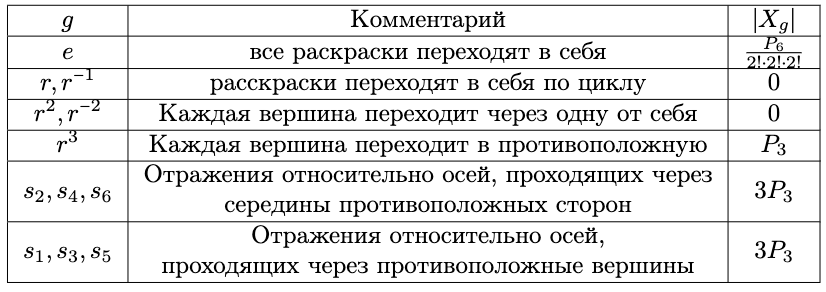
\includegraphics[width = 12.5cm]{Снимок экрана 2024-03-19 в 18.57.01.png}
\end{center}


По \textit{Лемме Бернсайда}: 

$$
\text{orb}(X) = \frac{\Sigma_{g \in G} |X_g|}{|G|} = \frac{90 + 0 + 0 + 6 + 18 + 18}{12} = 11
$$
\begin{center}
    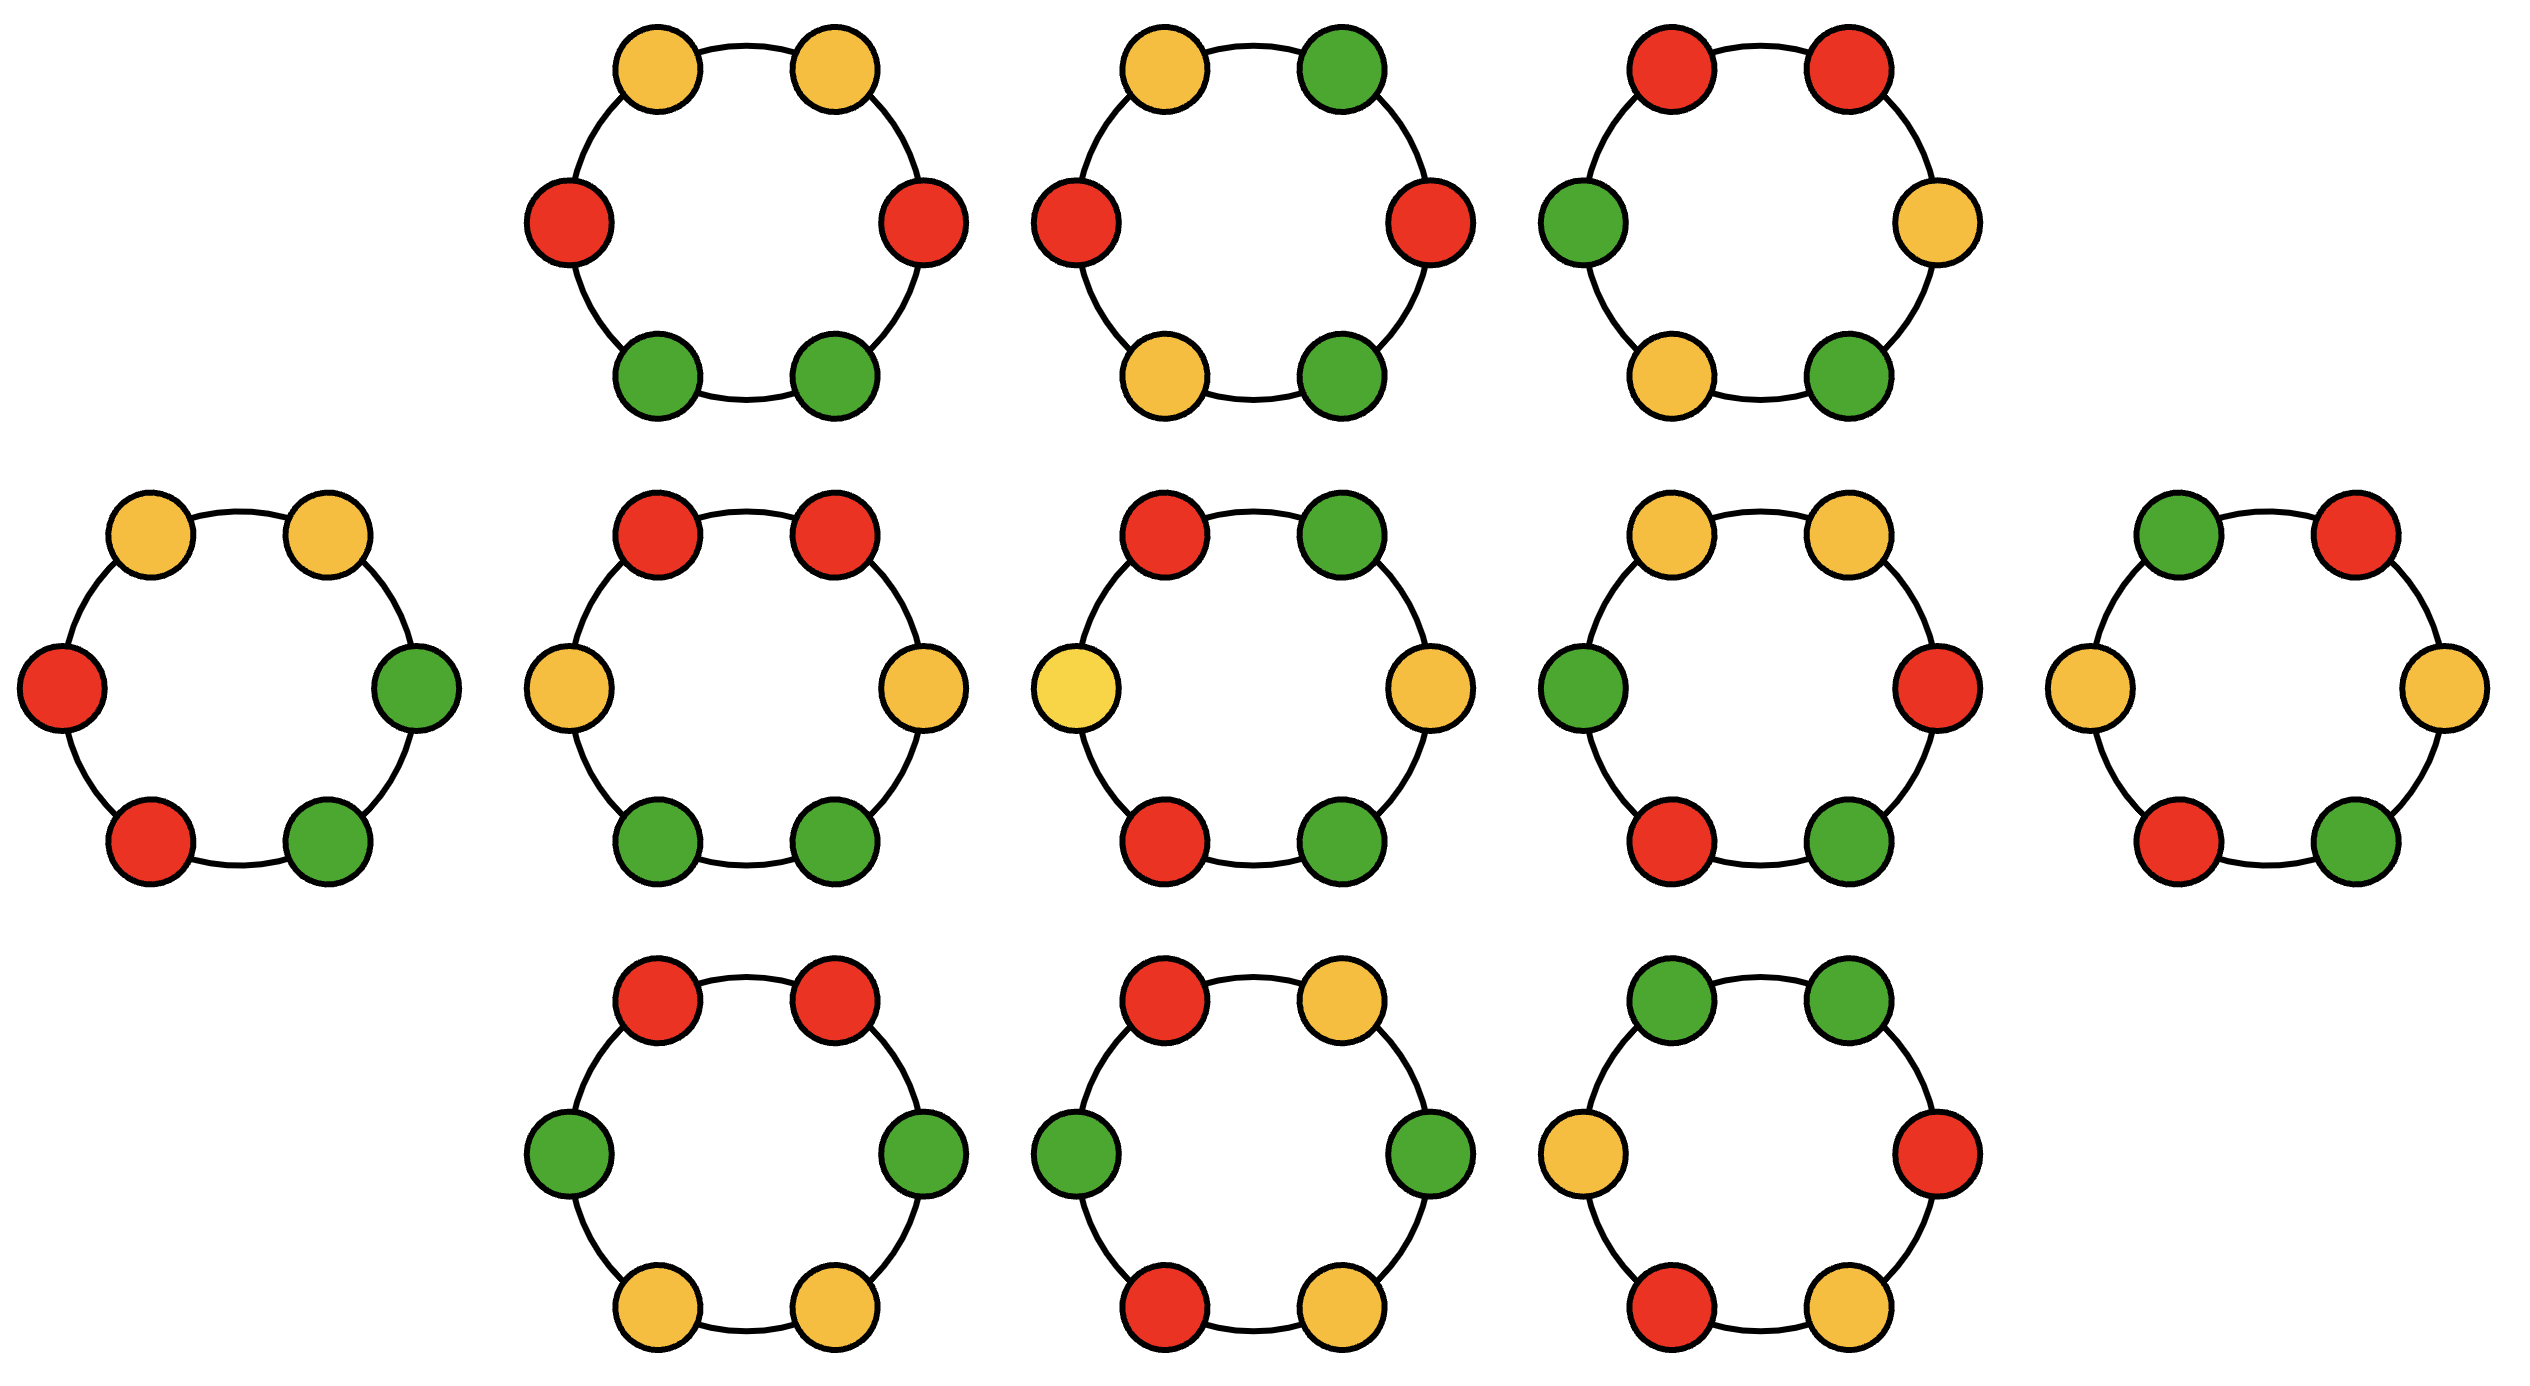
\includegraphics[width = 7 cm]{Снимок экрана 2024-03-19 в 18.52.29.png}
\end{center}
\end{solution}
\end{document}
